\subsubsection{UC6 - Attivazione login automatico}
\begin{figure}[h]
	\centering
	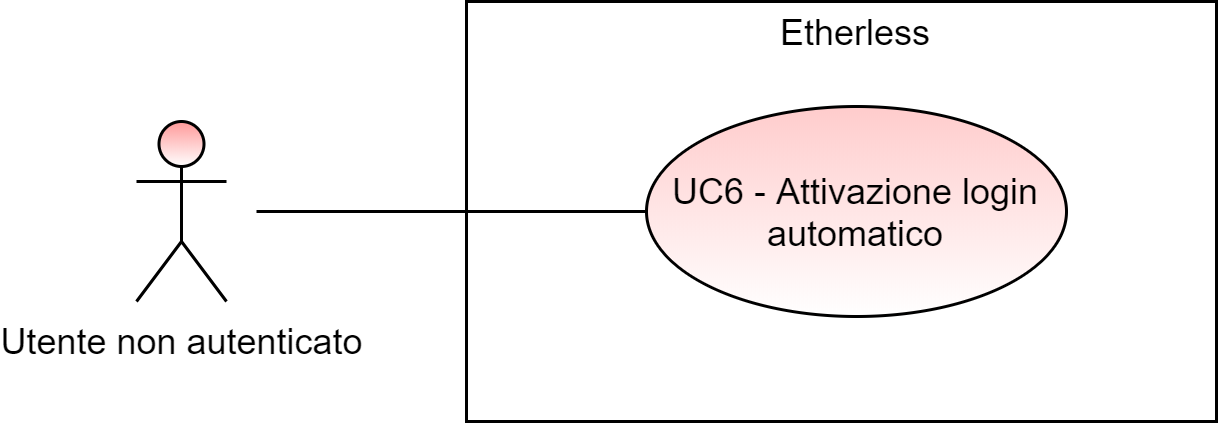
\includegraphics[scale=\ucs]{./res/img/UC6G.png}
	\caption {UC6 - Attivazione login automatico: schema generale}
\end{figure}
\begin{itemize}
	\item \textbf{Attori primari:} \una{};
	\item \textbf{Descrizione:} dopo aver inserito le credenziali di accesso l’utente specifica, tramite l’apposito flag \texttt{-r}, la richiesta di essere ricordato anche per eventuali accessi futuri;
	\item \textbf{Scenario principale:} 
	\begin{itemize}
		\item l’utente inserisce il comando di login seguito dalle credenziali necessarie e dal flag \texttt{-r};
		\item a seguito di una corretta autenticazione le credenziali dell’utente vengono salvate per gli accessi futuri.
	\end{itemize}
	\item \textbf{Precondizione:} l’utente richiede di attivare il login automatico tramite il flag \texttt{-r};
	\item \textbf{Postcondizione:} le informazioni necessarie all’autenticazione dell’utente vengono salvate correttamente in vista di accessi futuri.
\end{itemize}